\documentclass[tikz]{standalone}

\usepackage{tikz}
\usetikzlibrary{matrix, fit, positioning}


% see http://www.texample.net/tikz/examples/colorful-tables/
% see http://tex.stackexchange.com/questions/1111/problem-with-defining-shortcuts-for-tikz-matrices

\newcommand{\connectionsMatrix}[2][]{
  \def\x{$\bullet$}
  \matrix (#2) [#1, matrix of nodes, nodes in empty cells,
    ampersand replacement=\&,
    column sep=0pt, row sep=0pt, inner sep=0pt,
    nodes={ draw, color=lightgray, text=black, minimum size=1cm, anchor=center },
    column 1/.style={nodes={draw=none}},
    row 1/.style={nodes={draw=none}},
    ]{
         \& $p_1$ \& $p_2$ \& \dots \& $p_k$ \& \dots \& \dots \& $p_m$ \\
  $g_1$  \&       \&   \x  \&       \&       \&   \x  \&       \&   \x  \\
  $g_2$  \&   \x  \&       \&   \x  \&       \&   \x  \&   \x  \&       \\
  \vdots \&       \&   \x  \&       \&       \&   \x  \&   \x  \&       \\
  $g_i$  \&   \x  \&       \&   \x  \&   \x  \&       \&       \&       \\
  \vdots \&       \&       \&   \x  \&       \&   \x  \&       \&   \x  \\
  $g_n$  \&   \x  \&       \&       \&   \x  \&       \&   \x  \&   \x  \\
  };
}

\def\mminh{2}
\def\mmaxh{8}

\def\mminv{2}
\def\mmaxv{7}

\def\mmin{\mminh}
\def\mmax{\mmaxh}

% matrix, row, color
\newcommand*{\fith}[4][]{
  \def\m{#2}
  \def\i{#3}
  \def\color{#4}
  \node[fit=(\m-\i-\mmin) (\m-\i-\mmax), inner sep=-5pt, draw, color=\color, #1] {};
}

% matrix, column, color
\newcommand*{\fitv}[4][]{
  \def\m{#2}
  \def\j{#3}
  \def\color{#4}
  \node[fit=(\m-\mminv-\j) (\m-\mmaxv-\j), inner sep=-5pt, draw, color=\color, #1] {};
}


\newcommand{\used}[4]{
  \def\m{#1}
  \def\r{#2}
  \def\c{#3}
  \def\color{#4}
  \node[draw, cross out, color=\color, inner sep=5pt, thick] at (\m-\r-\c) {};
}
\newcommand{\usedv}[3]{\used{#1}{1}{#2}{#3}}
\newcommand{\usedh}[3]{\used{#1}{#2}{1}{#3}}



\begin{document}


\newcommand*{\showExtCoh}[4]{
  \def\m{#1}
  \def\i{#2}
  \def\j{#3}
  \def\ps{#4}

  \gdef\cohs{}
  \foreach \x in \ps { \global\edef\cohs{\cohs, coh(p_\x)} }

  \node[fit=(\m-\i-\mmin) (\m-\i-\mmax), inner sep=-5pt, draw, color=blue] {};
  \node[right=2pt of \m-\i-\mmax]
      {$ \mathrm{ext.\,coh.}(\tilde{c}_\j) = \Gamma\big( coh(g_\j) \cohs \big) $};
}

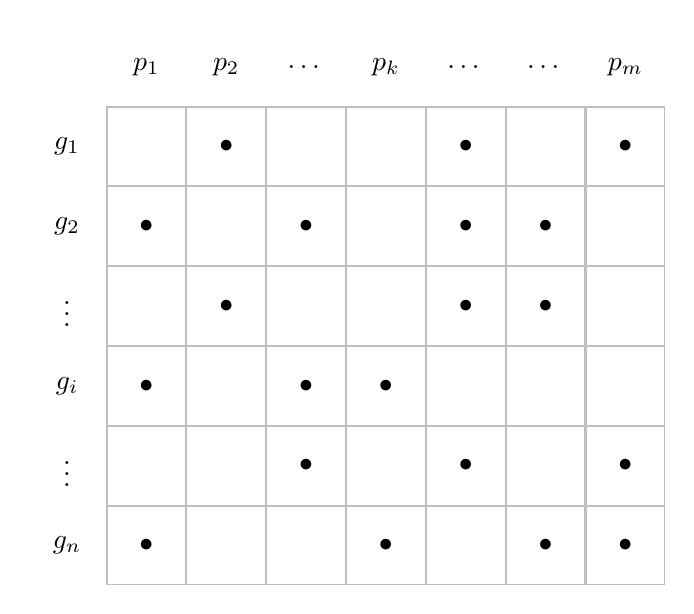
\begin{tikzpicture}

% Matrix - External coherence

\connectionsMatrix{m};

\showExtCoh{m}{2}{1}{2, *, m}
\showExtCoh{m}{3}{2}{1, *, *, *}
\showExtCoh{m}{4}{*}{2, *, *}
\showExtCoh{m}{5}{i}{1, *, k}
\showExtCoh{m}{6}{*}{*, *, m}
\showExtCoh{m}{7}{n}{1, k, *, m}



\end{tikzpicture}

\end{document}
